\section{Physical correction on a shared backbone}\label{app:matched-connection}
This physical-head-only study precedes geometric recovery. FM and GAGA use the same 2,381,566-parameter EGNN, 20,000 OMol25 rows, head architecture, and physical-supervision budget. Distance-self-conditioned FM receives 15,000 two-pass updates, matching the 960,000 example-forwards of GAGA's 30,000 one-pass updates (Appendix~\ref{app:feedback-transfer}). Each of two independent parents per method receives a separately fitted head.

\paragraph{Endpoint interface.}
Let $p$ denote schedule progress: flow time for FM and $1-t/t_{\max}$ for GAGA, with diffusion noise time $t$ and $t_{\max}=0.65$. The head takes $X$, predicted endpoint $H$, atom identities, and $p$, and predicts the bounded correction from Appendix~\ref{app:force-correction}. At strength $\eta$, the desired endpoint displacement is $\eta(1-p)A_\phi$. The native-output updates are
\begin{align}
 H=X+(1-p)v,
 &\qquad v^{\rm corr}=v+\eta A_\phi,
 \label{eq:matched-fm-correction}\\
 H=\frac{X-\sigma_t\epsilon}{\alpha_t},
 &\qquad \epsilon^{\rm corr}=\epsilon
       -\eta\frac{\alpha_t(1-p)}{\sigma_t}A_\phi.
 \label{eq:matched-gaga-correction}
\end{align}
Here $v$ is velocity, $\epsilon$ is predicted noise, and $\alpha_t,\sigma_t$ are signal and noise scales. Both updates induce the stated displacement. All parent tensors, native GAGA transitions, and observation noise remain fixed. With the common 16-element vocabulary, the head has 7,106 parameters and the same hidden pair network as the small FlowMol head.

\paragraph{Supervision and calibration.}
Each parent generates two trajectories on each of the same 128 training compositions, balanced across four atom-count ranges. Two late evaluations give 512 endpoints: FM progress 0.734375 and 0.921875, and the nearest GAGA progress values $1-174/650$ and $1-51/650$. All states receive mirror-paired, centered eSEN force labels and target $\delta(H)/(1-p)$. No target reaches the per-atom cap. Each head trains for 20,000 AdamW updates on 96 compositions; the other 32 assess prediction transfer. The four fits lower this error by 29.7--32.1\% relative to zero correction.

Eight separate validation compositions select one strength per algorithm across both fits from $\{0,1/4,1/2,1\}$. The criterion is joint yield at force RMS at most 5 eV/\AA, with ties favoring smaller strength. Both select $\eta=1$. We then fix the choice and evaluate 16 new compositions, eight each with 17--28 and 29--40 atoms, drawing 16 outputs per composition and fit. They are absent from the prepared training/validation corpora and earlier evaluation panels.

\begin{figure}[h]
\centering
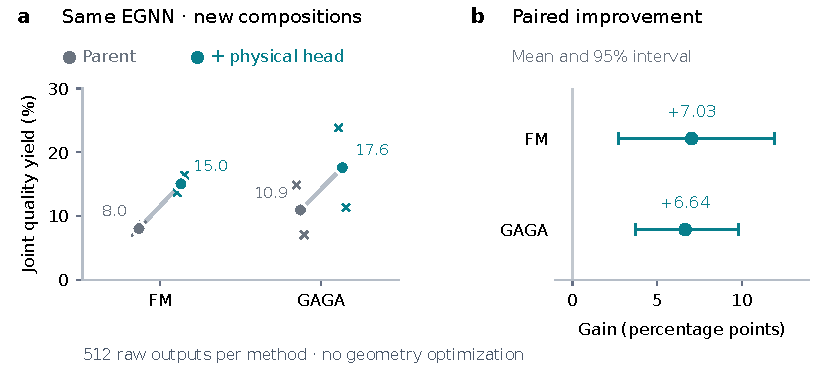
\includegraphics[width=\linewidth]{../research/figures/matched_connection_v1/matched_connection.pdf}
\caption{Physical correction transfers to independently trained EGNN generators.
(a) Joint yield requires an inferred valid graph and GFN2 force RMS at most
5 eV/\AA. Large circles show pooled rates; small crosses show the two fits.
(b) Within-parent improvements with paired composition-bootstrap 95\% intervals.
Both algorithms receive the same TRAIN compositions, force-query budget, head
architecture, and fitting schedule. All generated coordinates are unoptimized.}
\label{fig:matched-connection}
\end{figure}

\begin{table}[h]
\centering\small
\caption{Fresh shared-EGNN confirmation. Each row contains 512 attempts on the
same 16 compositions. The last two columns give joint yield in each independent
parent/head fit. Every GFN2 single-point calculation completed successfully.}
\begin{tabular}{lrrrr}
\toprule
Model & Graph (\%) & Joint (\%) & Fit 1 (\%) & Fit 2 (\%)\\
\midrule
FM, distance feedback &17.58&8.01&7.42&8.59\\
FM + physical head &20.31&15.04&13.67&16.41\\
GAGA &18.75&10.94&14.84&7.03\\
GAGA + physical head &20.31&17.58&23.83&11.33\\
\bottomrule
\end{tabular}\label{tab:matched-connection}
\end{table}

The primary FM comparison improves joint yield by 7.03 percentage points
(95\% interval $[2.73,11.91]$), with gains of 6.25 and 7.81 points in the two
fits. GAGA also benefits, gaining 6.64 points ($[3.71,9.77]$), with both fits
improving. Thus the learned correction transfers beyond the pretrained FlowMol
backbone and works with both velocity and noise prediction.

After identical physical supervision, FM minus GAGA is $-2.54$ points
($[-6.64,1.76]$). The difference between their within-parent improvements is
$+0.39$ points ($[-4.30,5.47]$). The experiment supports physical-head transfer
to both generators, while their ordering remains uncertain. Intervals resample
compositions and condition on the two fitted parents and heads; validation
strengths are fixed before test generation.


\paragraph{Cost and verification.}
Preparation uses 1,024 training trajectories, 4,096 eSEN queries, and 80,000 head updates. Validation and test each add 2,048 outputs and GFN2 calculations. Sampling uses 128 backbone calls plus 64 head calls for FM or 128 for GAGA. Zero-strength controls execute the same head operations. Head-supervision budgets match; FLOPs and runtime are not equated. Replay tests verify native sampling with zero heads and passive observers. Further checks reconstruct targets, measure fitted errors, reevaluate raw graphs, and independently parse xTB gradients. All reported outputs are generated without physical queries or optimization.

\subsection{Correction strength and the quality tradeoff}\label{app:connection-strength}
Because both methods selected the largest initial strength, we extend the grid to $\{0,1/4,1/2,1,2,4\}$ on the same eight validation compositions and random seeds. Only strengths two and four require new samples. Parents, heads, and labels are unchanged; the applied correction bound scales with $\eta$.

A conservative rule limits graph-validity losses relative to strength one to one pooled point and three points per fit. It retains strength one. A second rule, maximizing joint yield alone, selects strength four, with validation yields of 31.64\% for FM and 28.91\% for GAGA. This rule was introduced after the conservative screen but before new test generation. Both strengths are then evaluated on 32 previously ungenerated compositions, split equally between 17--28 and 29--40 atoms, with 16 draws per composition and fit.

\begin{table}[htbp]
\centering\small
\caption{Correction-strength comparison, with 1,024 raw outputs per row. Force is the median RMS among graph-valid, successfully scored outputs. Per-output sampling time is measured within the same GPU allocation for each fit, excluding loading and physical evaluation.}
\begin{tabular}{lrrrr}
\toprule
Model & Graph (\%) & Joint (\%) & Force (eV/\AA) & Time (s)\\
\midrule
FM, $\eta=1$ &20.12&15.14&3.833&0.123\\
FM, $\eta=4$ &22.17&20.80&3.159&0.122\\
GAGA, $\eta=1$ &20.80&16.50&3.805&0.143\\
GAGA, $\eta=4$ &21.00&20.02&3.158&0.143\\
\bottomrule
\end{tabular}\label{tab:connection-strength}
\end{table}

Increasing strength improves FM joint yield by 5.66 points (composition 95\% interval $[2.73,9.38]$), with fit-specific gains of 7.23 and 4.10. GAGA gains $+3.52$ points ($[0.00,7.52]$). At strength four, FM minus GAGA is $+0.78$ joint-yield points ($[-4.00,6.54]$) and $+1.17$ graph-validity points ($[-2.93,5.86]$). Joint differences of $-1.37$ and $+2.93$ across fits leave their ordering unresolved. FM samples 14.6\% faster in the recorded allocations, using 64 head calls rather than 128, with 128 backbone calls for both.

Over all outputs, stronger correction lowers FM mean GFN2 energy by 0.0622 eV/atom (signed-change interval $[-0.0769,-0.0479]$). Its strength-four energy remains 0.0527 eV/atom above GAGA ($[0.0273,0.0786]$). These within-composition comparisons include invalid outputs and different inferred connectivities. All graph-valid outputs have distinct canonical connectivities within each 16-draw composition/fit cell, ignoring stereochemistry.

Fragmentation dominates the remaining failures. At strength four, 533 of 1,024 FM outputs and 579 GAGA outputs fail contact connectivity. Only two FM outputs overlap at the specified threshold, both also disconnected; none of the GAGA outputs does. Among graph-valid outputs, 213/227 FM and 205/215 GAGA structures pass the force threshold. The extension adds 1,024 validation outputs and 4,096 confirmation outputs and GFN2 attempts, without new training or eSEN queries. One GAGA strength-one calculation fails and remains in the denominator; the other 4,095 succeed.

